\chapter{Introduction}\label{ch:Intro}
\section{Challenge, Motivation and Our Approach}
\label{sec:1}
\par The remarkable success of cellular wireless communication technologies makes it possible for smartphones to be widely used, which generates dramatical demand increase for mobile broadband capacity every year \cite{index2013global, cerwall2011ericsson, pujol2011mobile}. As a result, the conventional cellular bands below 3 GHz are very crowded. With the severe shortage of conventional cellular bands, millimeter wave (mmWave), between $30$ and $300$ GHz, frequency spectrum has been considered as a key component to addressing the bandwidth deficiency in the next generation wireless communication network \cite{khan2011mmwave, pi2011introduction, rappaport2011state, pietraski2012millimeter, rangan2014millimeter}. The available spectrum at these higher frequencies can be easily 200 times as much as today's cellular allocations that are largely constrained to the prime RF under 3 GHz. Moreover, the small wavelengths of mmWave signals combined with low-power complementary metal-oxide-semiconductor (CMOS) radio-frequency (RF) circuits enable large numbers of miniaturized antennas to be placed in small dimensions. Usage of these multiple antenna systems make it possible to make electrically steerable arrays with very high gain to be fabricated at the Base Station (BS) or even in the cellphone \cite{doan2004design, zhang2009antenna, gutierrez2009chip, rajagopal2011antenna}. These hardware and system advances promise mmWave a bright future.
\subsection{Next Generation Cellular Network}
\label{subsec:1}
\par There are fundamental differences between the current cellular communication system and the mmWave communication system, in terms of high propagation loss and sensitivity to blockage. Applications running on top of the mmWave network require low delay and high capacity. With high capacity, mmWave can easily satisfy the capacity demand. However, fading can substantially affect the performance of a wireless communication system. In general, fading can be divided into two categories: large-scale fading and small-scale fading. Small-scale fading is caused by multipath propagation. Large-scale fading, which is also known as shadow fading, is caused by obstacles in the propagation path. Electromagnetic waves have a minimal ability to diffract around obstacles with a size significantly larger than its wavelength. Currently, the frequency used by the LTE system has longer wavelengths than mmWave. This makes it possible to overcome the shadow fading caused by small size obstacles. High-frequency mmWave has small wavelengths, which make it more sensitive to blockage caused by small size obstacles like buildings, trees and even nearby pedestrians or vehicles. Therefore, shadow fading  can cause significant received power loss and significantly deteriorate the performance of the next generation wireless communication system. MmWave channel can be severely vulnerable to shadowing resulting in outages, rapidly changing channel conditions and intermittent connectivity. This makes it more challenging for mmWave system to provide low delay. According to aforementioned characteristics of mmWave channel, tough challenges need to be solved in order to fully exploit its potential. 


\par Shadow fading can cause significant received power loss for a wide area. This will lead to lost connections, which is harmful to mobile users who are using real-time applications which require low delay. To fully utilize the high bandwidth of mmWave links, shadow fading needs to be mitigated. Cooperative communication is an efficient way to reduce outage and provide better Quality of Service (QoS) for a single-cell model. Deploy ultra-dense network is considered as an efficient way to mitigate shadow fading for a multi-cell system. In most cases, shadow fading is assumed to be temporally and spatially independent to simplify the analysis of the system performance. Obviously, this is not the real scenario, especially for next generation wireless communication network. For mmWave communication networks, the cell size will become mush smaller than current LTE cell size due to high propagation loss \cite{rangan2014millimeter}. When cell size becomes comparable with the size of obstacles that cause shadow fading, shadow fading cannot be considered as spatially independent. Correlated shadow fading will result in correlated outage events and long outage duration. These will downgrade the performance of the system in terms of long delay. This thesis focuses on investigating the system performance under correlated shadow fading and proposing methods to mitigate correlated shadow fading. Since there is no consensus on the standard mmWave channel, we discuss the system performance under correlated shadow fading of the legacy cellular spectrum frequency and suggest applying it to mmWave channel in the future. 

\par With non-correlated shadow model, we can only analyze a snapshot of the system. However, in order to predict application performance over time, such as outage durations, correlated shadow fading model is necessary. At first, we choose distance-angle correlation model \cite{szyszkowicz2010feasibility} for shadow fading and investigate the correlated shadow fading problem in a single-cell cellular network. We find that correlated shadow fading could lead to correlated outage events and long outage durations.  To mitigate shadow fading and decrease shadow durations, wireless relays can be deployed. The performance of three different relay deployments with different relay densities is investigated. Theoretical analysis and simulations of outage performance are compared between different relay placement scenarios. The next generation wireless communication networks will be a dense multi-cell network \cite{rangan2014millimeter}, hence single-cell model is not adequate for analyzing next generation wireless communication networks. Interference will affect every receiving channel. Therefore, extending the investigation to a multi-cell network is necessary. When considering a multi-cell system, exponential correlated shadow fading model is used due to its popularity and simplicity. 

\par Exponential correlation model \cite{gudmundson1991correlation} has been widely used by researchers. Considering a single-cell model, exponentially correlated shadow fading can be modeled as a first-order autoregressive process. Given this feature, a first-order Markov chain model is developed and validated  to simplify the analysis. The Markov chain model is constructed by partitioning the entire shadow fading range into a finite number of intervals. The state transition matrix of the Markov chain is derived from the joint probability distribution of correlated log-normal shadow fading. Based on the proposed Markov chain model, the frequency and duration of outage near the edge of a single cell can be analyzed. To validate the Markov chain model, correlated Gaussian random fields can be simulated to analyze the outage frequency and durations due to correlated shadow fading. 
%Comparing the simulation results with the Markov chain model results, we conclude \reminder{Don't show your results, intro should be a place to tell people why the things you are going to talk about is important, and how you plan to do it, instead of results.} that the proposed Markov chain model is an efficient way to describe the channel variations, and the user experienced outage behavior of the channel. 
This Markov chain model can not be extended to multi-cell system because of the existing of interference from other base stations (BSs) and the co-existing of shadow fading auto-correlation and cross-correlation. To further elaborate the performance of multi-cell system and mitigate the correlated shadow fading, we run simulations for different BS densities. We believe increasing BS density will improve the system performance under correlated shadow fading. Two scenarios are investigated: MU connecting to the nearest BS and MU connecting to the BS with the strongest signal. We calculate signal-to-noise-and-interference ratio (SINR) for the mobile user (MU) with regard to different scenarios. Outage probability and outage duration can be generated from the SINR result. We find that increasing BS densities can decrease outage probability when MU is connected to the nearest BS. Outage duration will decrease when increasing the BS density in both cases. 

\par As we have mentioned above, mmWave channel provides a tremendous amount of capacity and relatively low delay while it suffers high propagation loss and sensitivity to blockage. Simulations and measurements revealed that the capacity gain is significant comparing with current cellular systems in \cite{akdeniz2014millimeter,bai2015coverage}. The last hop wireless channel capacity is not a bottleneck problem anymore. Meanwhile, mmWave channels are prone to variations due to the blockage from walls, trees, or even human body \cite{lu2012modeling, zhao201328, alejos2008measurement}. This feature brings frequent capacity variations to the channel. Typically, the channel switches periodically between two states: Line-of-Sight (LOS) and Non-Line-of-Sight (NLOS). The upper layer channel provided by mmWave communication network is not yet standardized; however, in general, there is a consensus that 5G mmWave channel will provide high capacity and low latency with frequent capacity fluctuation. For 5G mmWave wireless communication network, the legacy Transmission Control Protocol (TCP) might not work well due to the slow congestion detection and conservative loss recovery. Therefore, designing a new TCP congestion control scheme without involving any intermediate network device is necessary. In order to investigate existing TCP performance, a GINI testbed based link layer model is employed. This model is based on an Ethernet channel with high capacity and low delay. We extended the model to allow the physical link to be periodic on-off to mimic the mmWave channel where on means LOS and off denotes NLOS. Existing TCP congestion control protocols are tested on this channel. Both throughputs and the variation of congestion windows are shown with regard to different channel behaviors. A data-driven fast congestion prediction algorithm is proposed based on the idea of Explicit Congestion Notification (ECN). This fast congestion prediction algorithm can be utilized to design next generation transport layer protocols.
\subsection{Correlated Shadow Fading Models}
\label{subsec:2}
\par In most cases, shadow fading is modeled as an independent log-normal distribution \cite{goldsmith2005wireless} with a standard deviation derived from empirical measurements. An independent log-normal shadowing model is used widely when shadow fading cannot be ignored. But this model fails to capture the spatial correlations in shadow fading, which has been proved to be not negligible in \cite{graziano1978propagation}, \cite{marsan1990shadowing} and \cite{liberti1992statistics}. In \cite{szyszkowicz2010feasibility}, the author elaborated several models for correlated shadow fading,  investigated their feasibility and presented the physical plausibility of each model. Correlations can be divided into two categories: autocorrelation and cross-correlation as in Figure \ref{fig:1}. Autocorrelation is the correlation between two receivers receiving signal from the same transmitting node. Cross-correlation considers two transmitting nodes sending data to the same receiver. Autocorrelation and cross-correlation are symmetric in a mathematical sense and can be investigated in the same manner.
\begin{figure} 
\centering
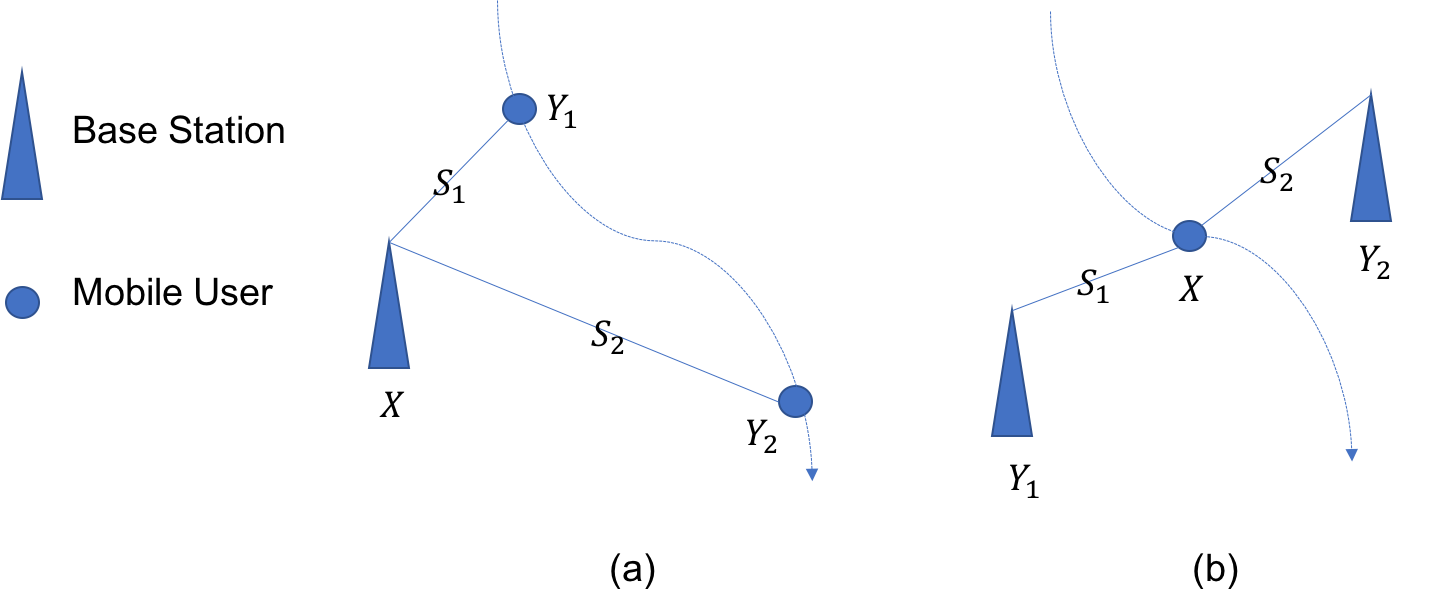
\includegraphics[width=14cm]{correlation.png}
\caption{(a) Shadowing autocorrelation for a mobile user, (b) Shadowing cross-correlation for a mobile user}
\label{fig:1}
\end{figure}
\par Autocorrelation and cross-correlation models can be described as in Figure \ref{fig:2}. There are $N$ points $Y_{1}, \cdots, Y_{N}$.  $S_{i}$ is the logarithm of the power attenuation due to shadowing on each path $\vec{r_{i}}$. $\mathbb{E}\{S_{i}\} = 0$ since shadow fading has correlated log-normal distribution. The log-variance of shadow fading can be characterized as 
\begin{equation}
\sigma_{i}^{2} = \mathbb{VAR}\{S_{i}\} = \sigma_{S}^2(\vec{r_{i}})
\label{eq:1}
\end{equation}
\begin{figure} 
\centering
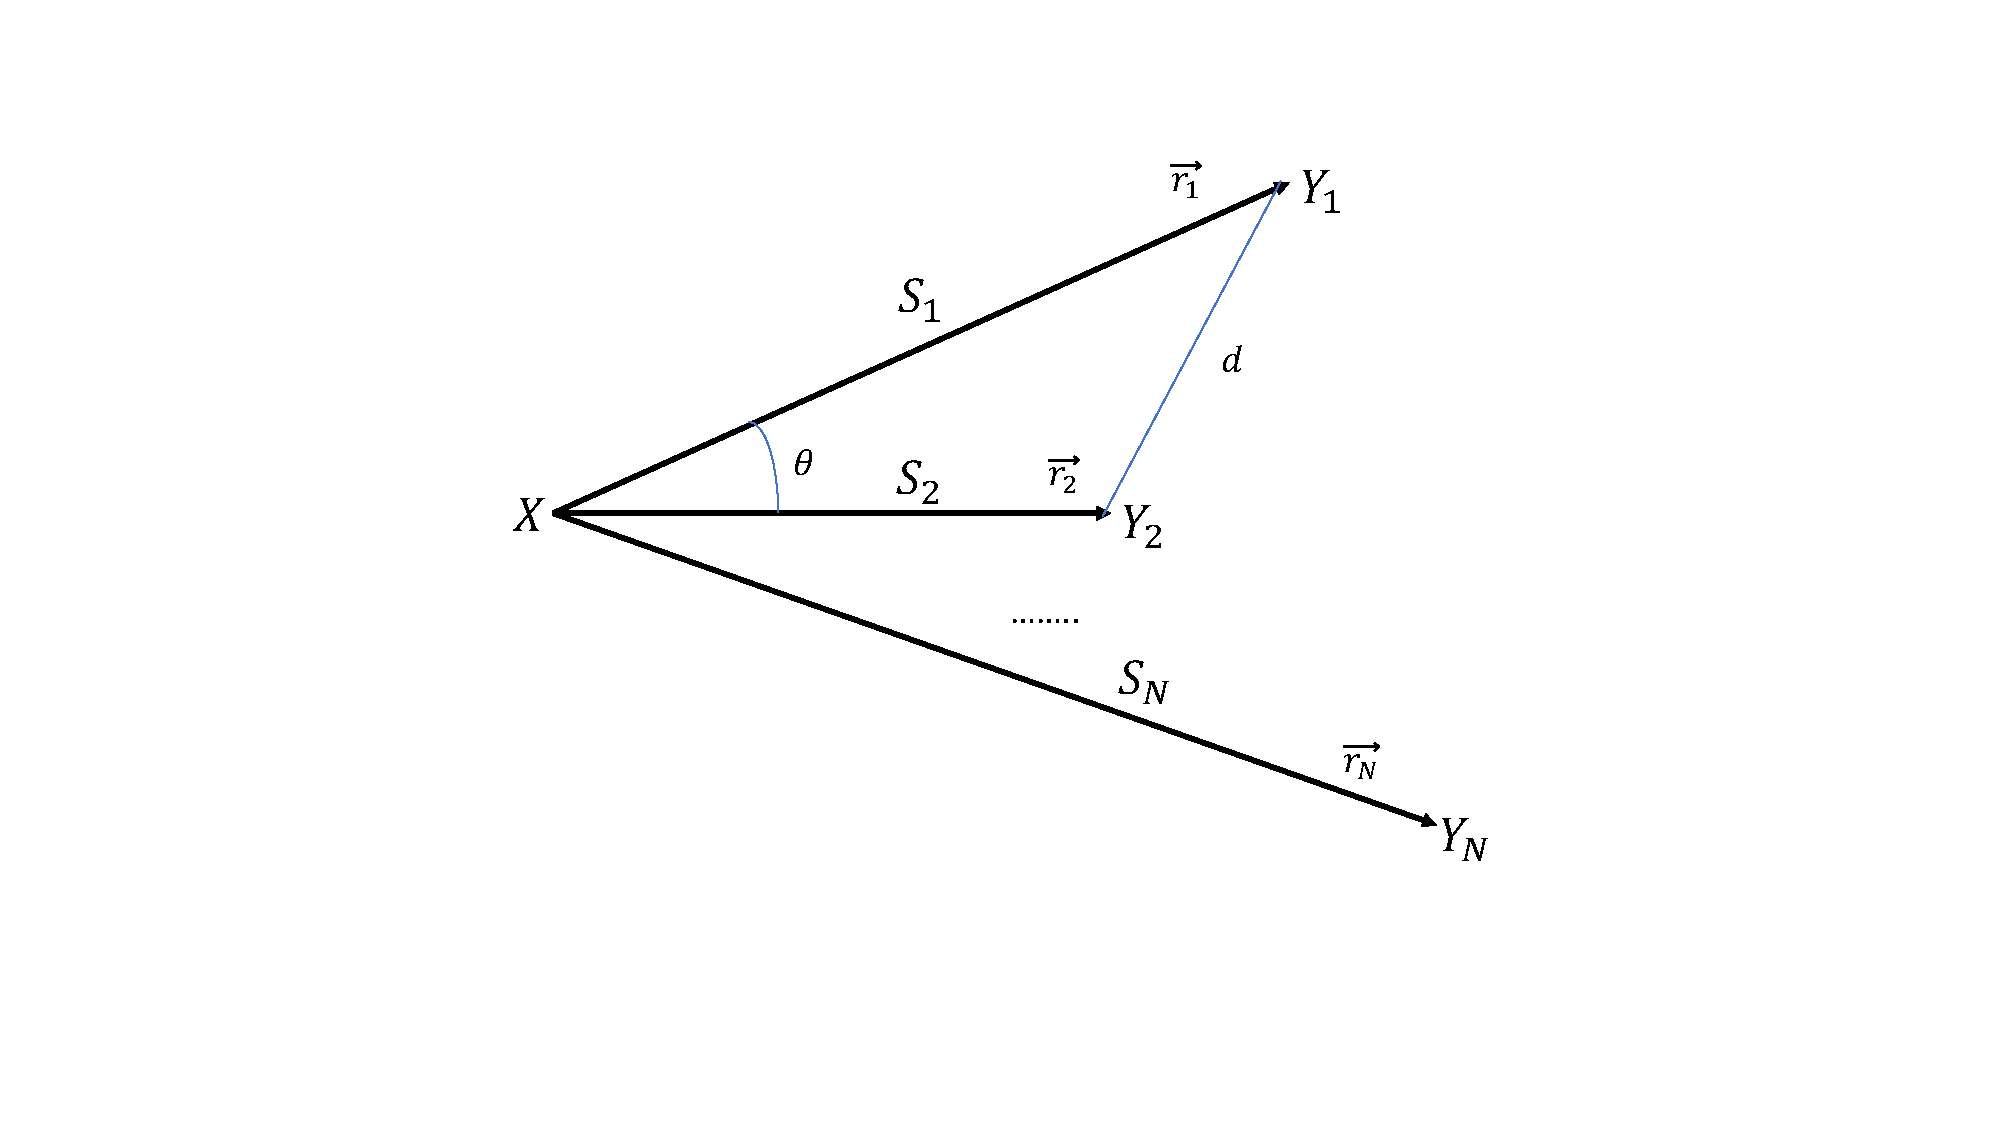
\includegraphics[width=14cm]{FadingGeometry.pdf}
\caption{Generic geometry of shadowing autocorrelation and cross-correlation}
\label{fig:2}
\end{figure}
This variance is considered as constant after a certain distance \cite{kitchener2006correlated}.
\par The correlation coefficients can be defined as
\begin{equation}
\begin{split}
& \rho_{i,j} = \mathbb{E}\{S_{i}S_{j}\}/\sigma_{i}\sigma_{j} = h(\vec{r_{i}}, \vec{r_{j}}), i \neq j \\
& \rho_{i,i} = 1.
\end{split}
\label{eq:2}
\end{equation}
The following properties will be held:
\begin{itemize} 
\item $-1\leq h(\vec{r_{i}}, \vec{r_{j}}) \leq 1$
\item $h(\vec{r_{i}}, \vec{r_{j}})  = h(\vec{r_{j}}, \vec{r_{i}}) $
\end{itemize}
The correlation matrix of $\mathbf{S} = [S_{1}, \cdots, S_{N}]$ is:
\begin{equation}
\mathbf{K} = \left[\begin{array}{cccc}
\sigma_{1}^{2} & \sigma_{1}\sigma_{2}\rho_{1,2} & \cdots & \sigma_{1}\sigma_{N}\rho_{1,N}\\
\sigma_{1}\sigma_{2}\rho_{1,2} & \sigma_{2}^{2} & \cdots & \sigma_{2}\sigma_{N}\rho_{2,N}\\
\vdots & \ddots & \ddots & \vdots\\
\sigma_{1}\sigma_{N}\rho_{1,N} & \sigma_{2}\sigma_{N}\rho_{2,N} & \cdots & 1\\
\end{array}\right].
\label{eq:3}
\end{equation}
For $\mathbf{K}$ to be a valid covariance matrix, it is necessary that $\mathbf{K}$ is positive semidefinite(\emph{psd}).
\par By grouping the measurements along one variable in several ways, $h$ can be expressed as a function of a single variable in the following three forms:
\begin{itemize}
\item absolute distance (between $Y_{1}$ and $Y_{2}$): $d = \Vert \vec{r_{1}}- \vec{r_{2}}\Vert$ .
\item angle of arrival separation: $\theta = \vert\angle\vec{r_{1}}-\angle\vec{r_{2}}\vert\in [0^\circ, 180^\circ]$ 
\item arrival distance ratio (in decibels): $R=\vert10\log_{10}r_{1}/r_{2}\vert=(10/\ln 10)\vert \ln r_{1}-\ln r_{2}\vert$
\end{itemize}
A correlation model needs to satisfy as many as the following criteria to become a precise model:
\begin{itemize}
\item $h(\vec{r_{i}}, \vec{r_{j}}) \approx 1$ for $\vec{r_{i}}\approx \vec{r_{j}}$.
\item $h(\vec{r_{i}}, \vec{r_{j}}) \ll 1$ for $\Vert \vec{r_{i}}- \vec{r_{j}}\Vert\gg0$.
\item $h$ should be a nonincreasing function in $\theta$, $R$ and $d$.
\item $h$ should be nonnegative.
\item $h$ should be small for large $\theta$ and approach zero for $\theta\approx180^\circ$ when $r_{1}$ and $r_{2}$ are large.
\item Continuity: a small change in $\vec{r_{i}}$ should result in small change in $h(\vec{r_{i}}, \vec{r_{j}})$.
\item Correlation should not depend on $d$ only.
\end{itemize}
Considering the above criteria, the author of \cite{szyszkowicz2010feasibility} recommended a correlated shadow fading model with distance and angle in \cite{szyszkowicz2011interference}, and provided a fast simulation method to generate the correlated shadowing field. We use this model to analyze single-cell system performance and discuss how cooperative communication can help to mitigate shadow fading. 

\par After investigating the single cell system, we attempt to investigate multi-cell system performance. The aforementioned distance-angle model cannot be applied to this scenario. The distance-angle model is designed for single-cell system with a single BS at the center of the shadowing field. Therefore, it is not suitable for multi-cell system. Meanwhile, auto-correlation and cross-correlation co-exist in a multi-cell system, which further complicates the analysis of system performance. To simplify the analysis without losing of generality, the exponential correlated model is deployed. Exponential correlated model of shadow fading is the most widely used model. It can be modeled as a Markov chain model in the single-cell case. This Markov model can be used to simplify the analysis of system performance; however, it cannot be used to analyze the performance of multi-cell system due to the presence of interference. Simulations are run to study the outage probability and outage duration of the multi-cell system given different network topologies. 


\subsection{Transmission Control Protocol (TCP)}
\label{subsec:3}
\par TCP is the transport layer protocol that provides reliable connection-oriented and in-order delivery service to applications \cite{panwar2004tcp}. TCP uses error control, flow control and congestion control to achieve this. When incoming traffic demand to the network exceeds its capacity, congestion occurs and propagates to other connected networks. Congestions in the network can generate long delay and high packet loss rate. Due to fading, the mmWave cellular network might be unstable and continuously switching between LOS and NLOS states frequently, thus resulting in large variations in data rate. This behavior determines that mmWave cellular network is prone to congestion. Therefore, designing an efficient congestion control protocol is necessary for the next generation wireless communication network. There are two points to implement congestion control: end-to-end TCP congestion control and queuing discipline in the routers inside the network. In this thesis, we will concentrate on end-to-end TCP congestion control. Legacy TCP uses slow start, congestion avoidance and fast retransmit/fast recovery to adapt to congestion in the routers. The sender maintains two variables for congestion control: a congestion window size (\emph{cwnd}), which upper bounds the sender rate, and a slow start threshold (\emph{ssthresh}), which determines how the sender rate is increased. Initially, \emph{cwnd} increases exponentially until it reaches \emph{ssthresh}. After that, \emph{cwnd} increases roughly linearly. When congestion occurs, \emph{cwnd} is reduced to $1$ segment to avoid segment loss. 
\par TCP relies on implicit signals received from the receiver or the timer times out to learn the state of the network. There are two ways in which TCP can detect packet loss: 
\begin{itemize}
\item Retransmission timeout (RTO): For each sent TCP segment, the sender expects to receive an acknowledgement (ACK) from the receiver within some period of time (RTO). If the ACK to a particular segment is not received by the sender before retransmission timer expires, the segment is considered to be lost. 
\item Duplicate ACKs: If the receiver received out of order data segment, it cannot acknowledge the out of order segment. Instead, it will acknowledge the last contiguous segment it has received prior to the lost segment. Upon the reception of the duplicate ACKs, the sender is informed about the loss of the segment.
\end{itemize}
Both methods above require the sender to wait for a period of time before initiating retransmission (RTO or duplicate ACKs). 
\par Considering characteristics of the mmWave channel, legacy TCP is not necessary to be a good choice for next generation networks. TCP works for regular network, which is stable and the only variation is congestion. However, it will not work well with mmWave channel, which has an on-off behavior and result in lots of packet loss. The slow start will be too conservative for senders to fully utilize the channel capacity. Since low delay mmWave channel switches between LOS and NLOS fast and frequently, time out and duplicate ACKs might not indicate the network condition precisely due to the long waiting time. To investigate the existing TCP performance on the mmWave-like channel, we used high-capacity Ethernet channel with periodical on-off behavior to mimic the mmWave channel. TCP throughput of NewReno and Cubic \cite{grieco2004performance, ha2008cubic} is tested on this channel. 
\par There are also some non-TCP congestion control techniques including Random Early Detection (RED) \cite{lin1997dynamics}, Explicit Congestion Notification (ECN) \cite{ramakrishnan2001rfc} and so on. After investigating the legacy TCP performance on a mimic mmWave channel, we proposed an end-user TCP congestion prediction algorithm based on ECN. The key idea of ECN is to mark packets as congestion experienced when the routing queue is longer than a threshold instead of dropping them. When the receiver receives the marked packet, it responses with a marked ACK to inform the sender that congestion may occur in the router. TCP senders can adjust their rate of transmission based on their own congestion avoidance algorithm. Inspired by ECN, we proposed a data driven virtual ECN algorithm to predict network congestions without involving routers or receivers.
\section{Dissertation Outline}
\par This thesis is organized as follows. In Chapter \ref{ch:2}, we introduce the distance-angle correlated shadow fading model and investigate the system performance of a single cell cellular network. We explain that the correlated shadow fading could lead to correlated outage events and long outage durations. To mitigate the shadow fading, relays are deployed to work cooperatively with the BS. The performance of three different relay deployments with different relay densities are discussed. Theoretical analysis and simulations of outage performance are given to compare between different relay placement scenarios. 
\par In Chapter \ref{ch:3}, the most widely used shadow fading correlation model: exponential correlation model is introduced. A Markov chain model is constructed for the spatially exponentially correlated shadow fading. This model can be used to analyze the outage behavior for a single cell system. We demonstrated that a well designed Markov chain model with an appropriate number of states corresponding to the standard deviation of the shadow fading is indeed a powerful tool to study system performance.
\par In Chapter \ref{ch:4}, we extend the system performance analysis under exponentially correlated shadow fading from a single-cell system to a multi-cell system. We compare two different BS layout: Grid and Random model, and conclude that Grid model performs better than Random model. System performance is investigated in terms of outage probability and outage duration given different BS density and connection strategies. 
\par In Chapter \ref{ch:5}, we investigate the performance of legacy TCP on a mimic mmWave channel. The result suggests that legacy TCP is not well designed for next generation networks. We proposed a data driven machine learning congestion detection algorithm, which can predict network congestion with high precision when network topology does not change dramatically. In the future, a fast reacting congestion control algorithm can be designed based on this algorithm.
\par Chapter \ref{ch:6} concludes the thesis and discusses some future research directions.








